\section{建模与构建}
本章从表\ref{tab:functions}中选择三个代表功能展开：许盛凯负责的乘客预约选座、后台辅助调度，以及赵凯彭负责的司机任务与位置共享。每个功能均按场景建模、类建模、功能建模/行为建模、代码结构及说明、界面截图的顺序给出阶段结果。建模围绕现有 Dart 类和控制器方法展开，突出业务规则与实现之间的对应关系。

\subsection{功能一 乘客预约选座与订单管理}
\owner{许盛凯}
该功能将车次容量、座位占用、重复预约和订单状态约束集中到状态控制器，是乘客端最主要的交互流程。其难点在于页面显示的可选座位必须与创建预约时的校验保持一致，取消操作还会同时影响座位、信用分和通知。

\subsubsection{场景建模}
\begin{table}[H]\centering\small
\caption{乘客预约选座用例描述}
\begin{tabularx}{\linewidth}{|P{2cm}|Y|}\hline
用例名称 & UC-P01 预约车次并选择座位\\\hline
参与者 & 已登录的普通用户\\\hline
前置条件 & 用户进入普通用户工作台；目标车次处于待发车状态且发车时间晚于当前时间。\\\hline
触发事件 & 用户在车次卡片点击预约，进入选座对话框。\\\hline
基本流程 & （1）查看路线、时间、费用和余座；（2）打开选座界面；（3）选择可用座位；（4）确认预约；（5）控制器校验车次、余座、重复预约和座位有效性；（6）创建待发车、待支付的预约；（7）刷新列表并生成预约通知。\\\hline
异常流程 & 车次不可预约、余座为零、同一用户已有该车次有效预约或所选座位不可用时，返回具体原因，不新增预约。\\\hline
后置条件 & 新预约进入个人预约列表；该座位从可用座位集合中移除，车次显示余座相应减少。\\\hline
关联操作 & 模拟支付更新支付状态；发车前取消预约释放占座并扣减信用分。\\\hline
\end{tabularx}\end{table}
预约、支付和取消分别由独立操作触发。订单的业务状态与支付状态分开保存：支付成功后订单仍为待发车状态，不将“已支付”作为行程结束。取消仅允许待发车预约，且车次不能已发车。

\subsubsection{类建模}
图\ref{fig:passenger-class}保留与预约直接相关的核心字段。用户与车次通过预约关联，支付记录通过预约标识与订单关联；控制器管理状态，页面只调用操作并展示结果。
\begin{figure}[H]\centering
\begin{tikzpicture}[x=1cm,y=1cm]
\node[box,text width=5.9cm] (trip) at (0,0) {\textbf{TripModel}\par\rule{5.7cm}{0.3pt}\par\code{id, departureTime, totalSeats}\par\code{bookedSeats, fare, status}\par\code{isBookable}};
\node[box,text width=5.9cm] (user) at (7.3,0) {\textbf{UserModel}\par\rule{5.7cm}{0.3pt}\par\code{id, name, phone}\par\code{role, creditScore}\par 用户身份与信用状态};
\node[box,text width=5.9cm] (booking) at (0,-4.0) {\textbf{BookingModel}\par\rule{5.7cm}{0.3pt}\par\code{id, userId, tripId, seatNo}\par\code{status, fare, paymentStatus}\par\code{isActive, canPay, copyWith()}};
\node[box,text width=5.9cm] (pay) at (7.3,-4.0) {\textbf{PaymentModel}\par\rule{5.7cm}{0.3pt}\par\code{id, bookingId, amount}\par\code{method, status}\par\code{createdAt, completedAt}};
\draw (trip.south)--node[font=\scriptsize,right,pos=.15]{1}node[font=\scriptsize,right,pos=.85]{0..*}(booking.north);
\draw (user.south)--node[font=\scriptsize,right,pos=.15]{1}node[font=\scriptsize,right,pos=.85]{0..*}(booking.north east);
\draw (booking.east)--node[font=\scriptsize,above]{1\quad 0..*}(pay.west);
\end{tikzpicture}
\caption{乘客预约核心类模型（字段节选，关联通过标识保存）}\label{fig:passenger-class}
\end{figure}

\noindent\textbf{模型约束。}有效预约由\code{BookingModel.isActive}判定，其条件是业务状态为\code{pending}。\code{TripModel.isBookable}同时检查车次状态与发车时间。Mock 数据中\code{bookedSeats}表示初始化时已有的占用座位，新增预约单独记录，因此计算余座时需要扣除两部分。

\subsubsection{功能建模/行为建模}
图\ref{fig:passenger-sequence}展示从用户确认选座到状态刷新和本地通知的关键顺序。初始数据由仓库提供，实际创建预约时直接读取当前内存状态，无网络请求。
\begin{figure}[H]\centering
\begin{tikzpicture}[x=1cm,y=1cm,font=\small]
\node[box,align=center,text width=1.35cm] (u) at (0,0) {乘客};
\node[box,align=center,text width=2cm] (ui) at (3.0,0) {预约页面};
\node[box,align=center,text width=2.8cm] (c) at (7.0,0) {预约控制器};
\node[box,align=center,text width=2.0cm] (n) at (11.5,0) {本地通知状态};
\foreach \a in {u,ui,c,n} \draw[lifeline] (\a.south)--+(0,-6.8);
\draw[flow] (0,-1)--node[above,smalllabel]{选座并确认}(3,-1);
\draw[flow] (3,-2)--node[above,smalllabel]{createBooking(...)}(7,-2);
\draw[flow] (7,-2.55)--(7.8,-2.55)--node[right,font=\footnotesize,align=left]{校验车次、容量、\\重复预约、座位}(7.8,-3.5)--(7,-3.5);
\node[box,text width=5.6cm,font=\footnotesize,align=center] at (3.0,-4.0) {校验失败：返回原因，页面提示，不新增预约};
\draw[flow] (7,-4.8)--(8,-4.8)--node[right,font=\footnotesize]{创建预约并替换状态}(8,-5.4)--(7,-5.4);
\draw[flow] (7,-5.85)--node[above,smalllabel]{push 预约通知}(11.5,-5.85);
\draw[flow,dashed] (7,-6.6)--node[above,smalllabel]{返回操作结果 / 状态变化刷新 UI}(3,-6.6);
\end{tikzpicture}
\caption{预约创建的关键交互顺序}\label{fig:passenger-sequence}
\end{figure}

余座和座位集合的计算规则为：
\[
 R=T-B-\left|\{b\mid b.tripId=t.id\land b.isActive\}\right|,
\]
其中 $T$ 为车次总座位数，$B$ 为初始化占用数。可选座位从 $B+1$ 到 $T$ 枚举，再移除有效预约已使用的座位号。取消后预约不再属于有效集合，因此该座位可重新选择。

取消时，距发车时间不超过120分钟扣5分，其余扣2分；已发车时直接拒绝取消。模拟支付单独经历待支付、支付中和已支付状态。以上规则在控制器中统一处理，避免不同页面各自维护一套判断。

\subsubsection{代码结构及说明}
\begin{table}[H]\centering\small
\caption{预约功能代码结构与职责}
\begin{tabularx}{\linewidth}{|P{2.1cm}|Y|}\hline
层次 & 文件与职责\\\hline
页面层 & \code{lib/features/passenger/presentation/passenger_home_page.dart}：车次卡片、选座对话框、预约列表、取消确认与支付界面。\\\hline
状态层 & \code{lib/features/passenger/booking/providers/passenger_booking_provider.dart}：管理车次、预约、支付及业务操作结果。\\\hline
数据层 & \code{lib/features/passenger/booking/data/mock_passenger_repository.dart}：提供初始车次和预约。\\\hline
模型与公共状态 & \code{lib/core/models/booking_model.dart}、\code{trip_model.dart}、\code{payment_model.dart}；信用与通知分别由认证状态和通知状态管理。\\\hline
\end{tabularx}\end{table}

\noindent\textbf{核心方法。}\code{createBooking}依次检查业务条件，构造\code{BookingModel}，再以新列表更新状态；\code{cancelBooking}更新预约、扣减信用分并写入通知；\code{payBooking}创建支付记录并通过模拟延时更新结果。下面摘录创建预约的主要校验，省略返回消息和对象构造：
\begin{source}
if (!trip.isBookable) return failure;
if (state.remainingSeatsForTrip(tripId) <= 0) return failure;
if (state.hasActiveBooking(userId: userId, tripId: tripId)) {
  return failure;
}
if (!state.availableSeatsForTrip(tripId).contains(seatNo)) {
  return failure;
}
// Create BookingModel; replace state; push local notification.
\end{source}
\noindent 上述为控制流程摘要，\code{failure}代表实际代码中带具体消息的\code{BookingActionResult}。实现通过不可变对象与列表替换触发页面刷新，页面不直接修改模型字段。

\noindent\textbf{阶段验证。}已有测试覆盖创建预约、取消和模拟支付，以及同车次重复预约、重复取消和不可取消状态等规则。测试文件为\code{test/widget_test.dart}与\code{test/business_rule_test.dart}。下一阶段需要增加并发占座、支付与取消交叉操作的验证，并在共享服务端接入后使用事务保证跨设备座位一致性。

\clearpage
\subsubsection{界面截图}
\begin{figure}[H]\centering
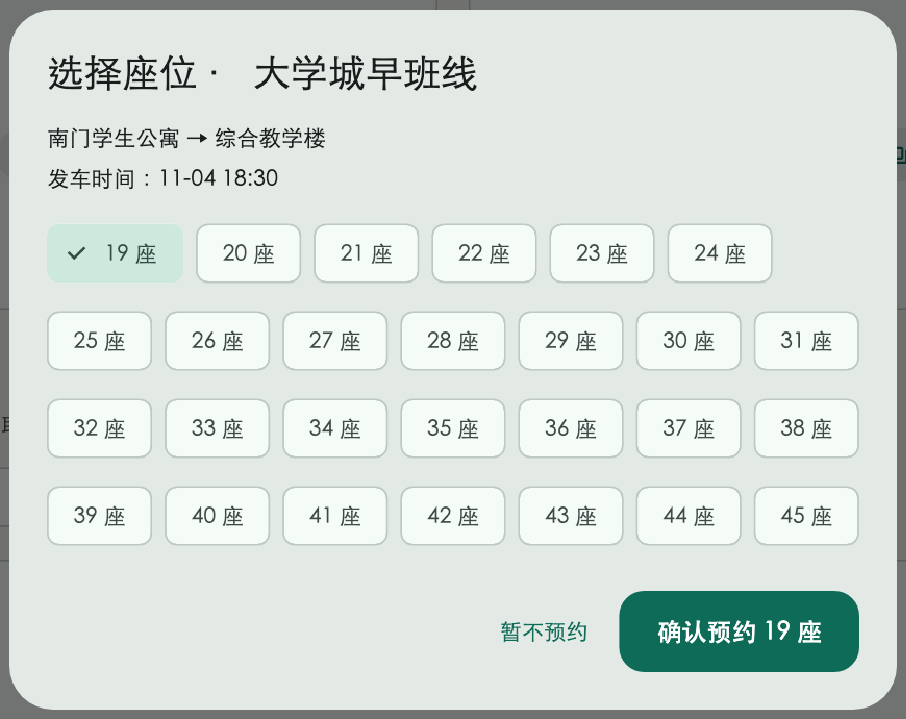
\includegraphics[width=12cm,height=0.64\textheight,keepaspectratio]{figures/passenger.pdf}
\caption{乘客选择19号座位并确认预约的运行界面}\label{fig:passenger-screen}
\end{figure}

界面将路线、发车时间、票价和余座放在同一车次卡片中，选座对话框提供明确的座位编号与可选状态。确认后，用户可以在“我的预约”中继续完成支付或取消，相关状态由同一预约模型驱动。

本阶段已完成从车次浏览到预约创建的本地交互流程，并补充了取消、信用和支付状态展示。后续将优先完善错误反馈和边界测试，再对接持久化与统一认证，保持预约规则在三端共享数据后的稳定性。
